\section{Model danych}

\subsection{Diagram związków-encji}

\begin{figure}[!htb]
  \begin{center}
    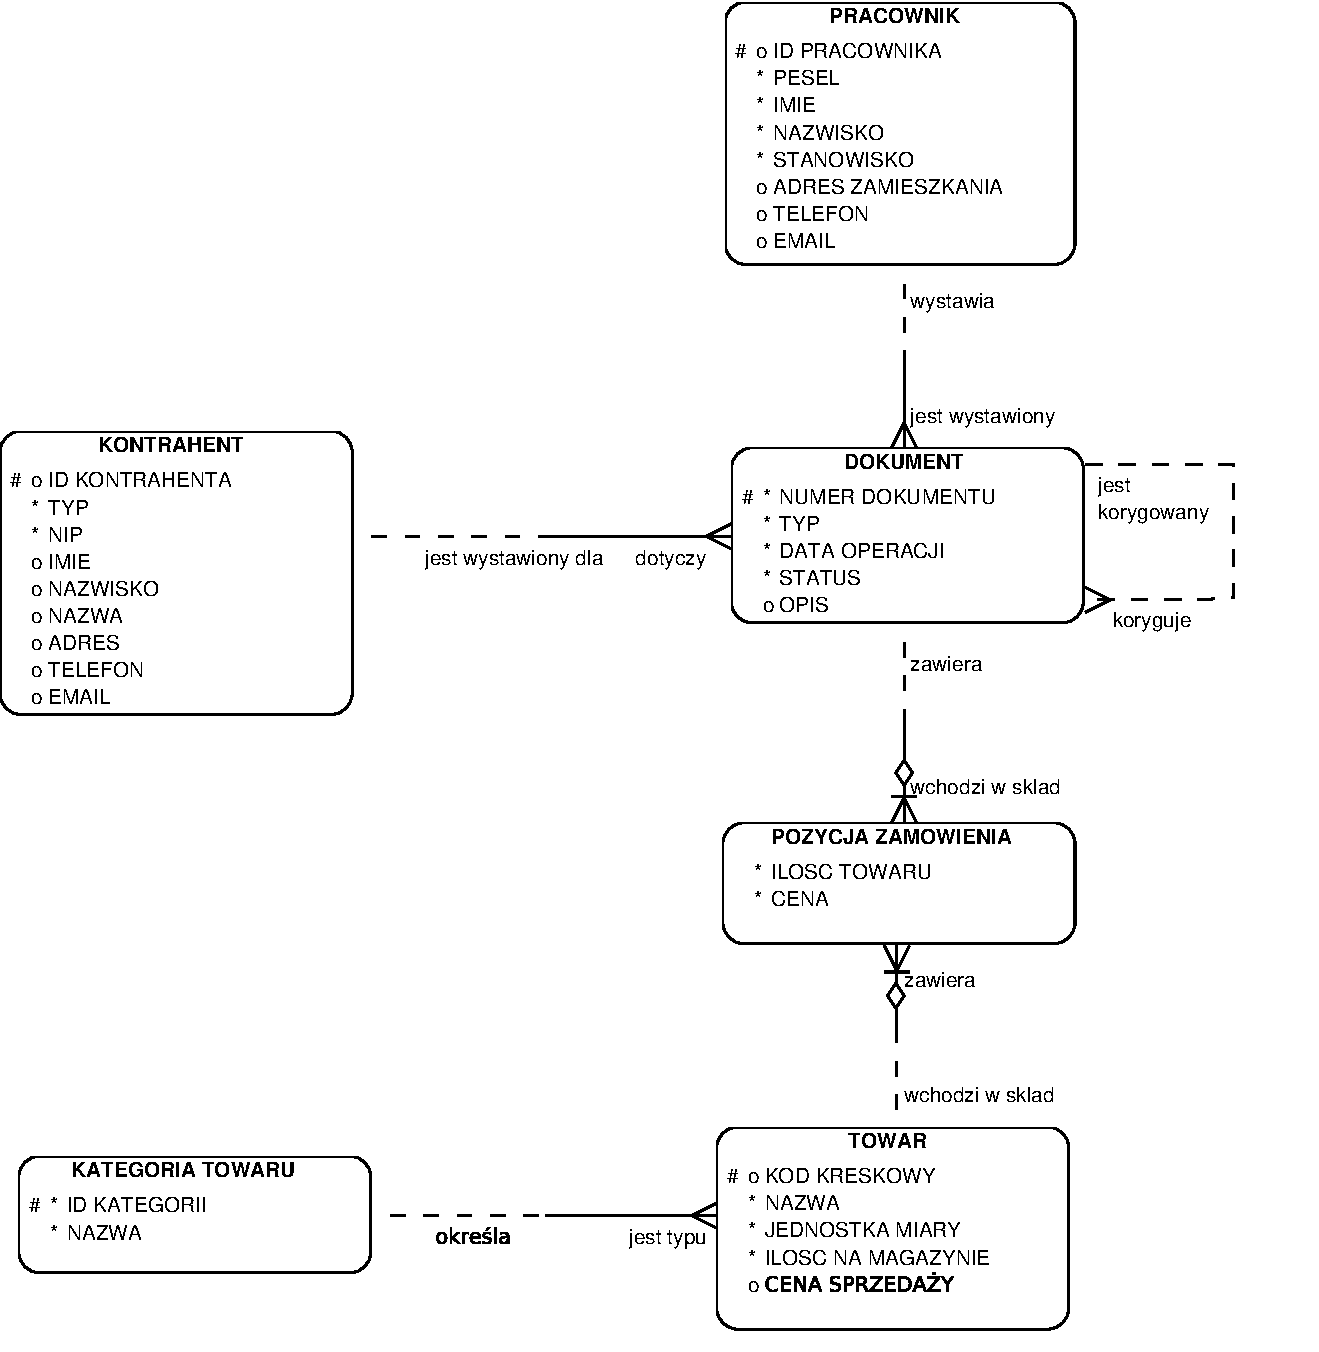
\includegraphics[scale=0.7]{../img/model/diagram_er_magazyn.pdf}
  \end{center}
  \caption{Diagram związków encji dla magazynu}
  \label{fig:magazyn-er}
\end{figure}
\FloatBarrier

\begin{figure}[!htb]
  \begin{center}
    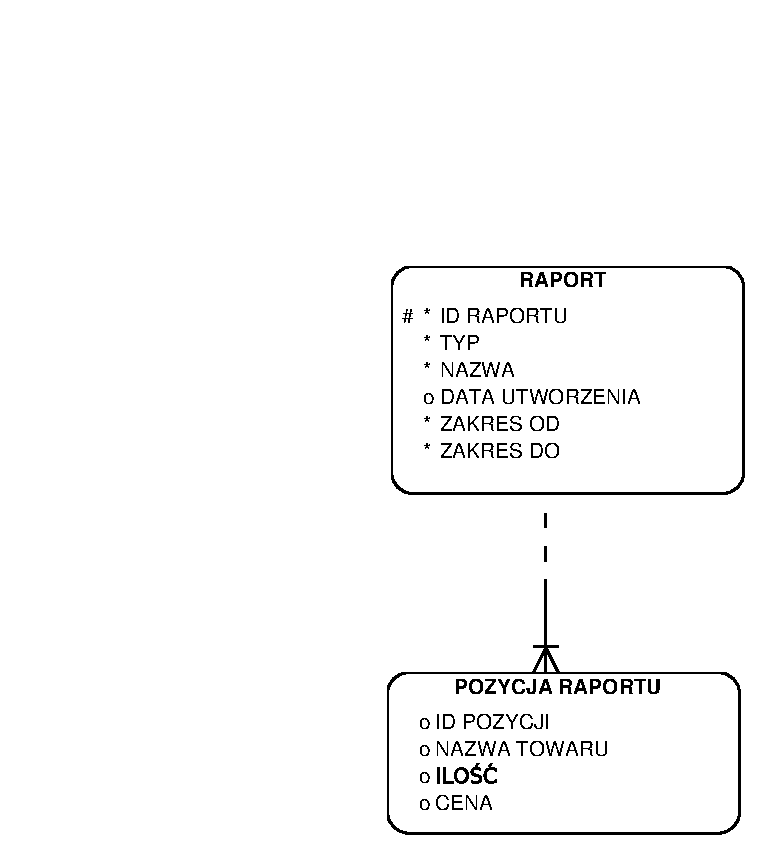
\includegraphics[scale=0.7]{../img/model/diagram_er_raporty.pdf}
  \end{center}
  \caption{Diagram związków encji dla tworzonych raportów}
  \label{fig:raport-er}
\end{figure}
\FloatBarrier

\subsection{Opis bazy danych}
W niniejszym podrozdziale znajduje się opis bazy danych przedstawionej na
rysunkach \ref{fig:magazyn-er} oraz \ref{fig:raport-er}.

\subsubsection{Tabela PRACOWNICY}
Tabela pracownicy zawiera informacje o pracownikach, którzy mogą używać
aplikacji do celów obsługi magazynu. Zostały w niej zawarte najważniejsze atrybuty jakie posiada każdy z
pracowników, takie jak:
\begin{itemize}
  \item \textbf{id\_pracownika} - sztuczny klucz główny, służy do identyfikacji
  pracownika w bazie danych, atrybut obowiązkowy
  \item \textbf{PESEL} - numer Powszechnego Elektronicznego Systemu Ewidencji
  Ludności pracownika, atrybut obowiązkowy
  \item \textbf{imie} - pierwsze imię pracownika, atrybut obowiązkowy
  \item \textbf{nazwisko} - nazwisko pracownika, atrybut obowiązkowy
  \item \textbf{stanowisko} - określa stanowisko na jakim pracuje pracownik,
  określa uprawnienia pracownika. Dopuszczalne stanowiska w systemie: magazynier,
  sprzedawca, kierownik. Atrybut obowiązkowy.
  \item \textbf{adres\_zamieszkania} - adres zamieszkania pracownika, atrybut
  opcjonalny
  \item \textbf{telefon} - numer telefonu pracownika, atrybut opcjonalny
  \item \textbf{email} - adres poczty elektronicznej pracownika, atrybut
  opcjonalny
\end{itemize}

W tabeli tej nie ma żadnych dodatkowych ograniczeń poza określeniem
obowiązkowości bądź opcjonalności atrybutów.

\subsubsection{Tabela DOKUMENTY}
Tabela ta reprezentuje dokumenty, które mogą być tworzone oraz przechowane w
systemie. Są to w szczególności dokumenty przyjęcia towarów, dokumenty wydania
na zewnątrz oraz korekty tych dokumentów. Każdy z dokumentów zawiera wymienione
poniżej atrybuty:
\begin{itemize}
  \item \textbf{numer\_dokumentu} - klucz sztuczny stanowiący unikalny
  identyfikator dokumentu, atrybut obowiązkowy
  \item \textbf{typ} - określa czy jest dokument przyjęcia czy też wydania
  towaru, atrybut obowiązkowy
  \item \textbf{data\_operacji} - określa datę stworzenia dokumentu w systemie,
  atrybut obowiązkowy
  \item \textbf{status} - określa stan w jakim znajduje się dokument, gdy
  dokument jest tworzony jego status to niezrealizowany, w momencie realizacji
  status zmienia swoją wartość na zrealizowany, a przy wystawieniu korekty
  dokument posiada status korekta, atrybut obowiązkowy
  \item \textbf{opis} - opis dokumentu w celach informacyjnych, atrybut
  opcjonalny
\end{itemize}

W tabeli tej oprócz standardowych ograniczeń opcjonalności oraz unikalności,
konieczne jest stworzenie wyzwalacza pilnującego aby dokument o statusie korekta
posiadał id korygowanego dokumentu.

\subsubsection{Tabela POZYCJE\_ZAMÓWIENIA}
Zawiera informacje o pozycjach występujących w stworzonym dokumencie. Pozycja
zamówienia posiada tylko dwa następujące atrybuty:
\begin{itemize}
  \item \textbf{ilosc} - zawiera informacje o ilości zamówionego bądź
  zamawianego towaru, atrybut obowiązkowy
  \item \textbf{cena} - określa cenę towaru, atrybut obowiązkowy
\end{itemize} 

Tabela nie posiada żadnych dodatkowych ograniczeń poza opcjonalnością.

\subsubsection{Tabela TOWARY}
Tabela towary opisuje towary przechowywane w magazynie. Posiada następujące
atrybuty:
\begin{itemize}
  \item \textbf{kod\_kreskowy} - kod EAN (\textit{ang. European Article
  Number} Europejski Kod Towarowy) towaru, atrybut obowiązkowy
  \item \textbf{nazwa} - nazwa towaru, ułatwiająca pracownikowi zidentyfikowanie
  towaru, atrybut obowiązkowy
  \item \textbf{jednostka\_miary} - jednostka miary w jakiej wyrażona jest ilość
  towaru, atrybut obowiązkowy
  \item \textbf{ilosc\_w\_magazynie} - określa ilość towaru znajdującego się w
  danej chwili w magazynie, atrybut obowiązkowy
  \item \textbf{cena\_sprzedazy} - określa sugerowaną cenę sprzedaży towaru,
  atrybut opcjonalny ponieważ mogą istnieć towary których cena sprzedaży w
  momencie dostawy jest nieokreślona
\end{itemize}

Tabela nie posiada żadnych dodatkowych ograniczeń poza opcjonalnością oraz
unikalnością nazwy.

\subsubsection{Tabela KATEGORIE\_TOWARÓW}
Tabela kategorie towarów przechowuje informacje o  kategoriach jakii mogą być
towary w magazynie.
Posiada ona tylko dwa atrybuty obowiązkowe:
\begin{itemize}
  \item \textbf{id\_kategorii} - sztuczny klucz identyfikujący kategorie,
  atrybut obowiązkowy
  \item \textbf{nazwa} - nazwa kategorii, atrybut obowiązkowy
\end{itemize}

Tabela nie posiada żadnych dodatkowych ograniczeń poza opcjonalnością oraz
unikalnością nazwy i klucza.

\subsubsection{Tabela KONTRAHENCI}
Tabela kontrahenci reprezentuje osoby fizyczne bądź firmy z którymi
współpracuje magazyn, mogą być to zarówno dostawcy jak i klienci magazynu. Kontrahent opisany
jest za pomocą następujących atrybutów:
\begin{itemize}
  \item \textbf{id\_kontrahenta} - sztuczny klucz główny identyfikujący
  kontrahenta w bazie danych, atrybut obowiązkowy
  \item \textbf{typ} - typ kontrahenta, dopuszczalne typy to dostawca oraz
  klient, atrybut obowiązkowy
  \item \textbf{imie} - imię kontrahenta w przypadku gdy kontrahentem jest osoba
  fizyczna, atrybut opcjonalny
  \item \textbf{nazwisko} - nazwisko kontrahenta w przypadku gdy jest nim osoba
  fizyczna, atrybut opcjonalny
  \item \textbf{nazwa} - nazwa kontrahenta w przypadku gdy jest nim
  przedsiębiorstwo, atrybut opcjonalny 
  \item \textbf{adres} - adres siedziby kontrahenta, atrybut opcjonalny
  \item \textbf{telefon} - numer telefonu kontrahenta, atrybut opcjonalny
  \item \textbf{email} - adres poczty elektronicznej kontrahenta, atrybut
  opcjonalny
\end{itemize}

Oprócz standardowych ograniczeń takich jak: opcjonalność oraz unikalność,
konieczne jest stworzenie wyzwalacza panującego nad prawidłową nazwą
kontrahenta. Zadaniem tego wyzwalacza powinno być sprawdzenie czy użytkownik
podał imię i nazwisko (w przypadku osoby fizycznej) bądź nazwę (w przypadku
przedsiębiorstwa). Wyzwalacz będzie uruchamiany w momencie dodawania i aktualizacji danych kontrahenta.

\subsubsection{Tabela RAPORTY}
Tabela raporty umożliwia kierownikom śledzenie ilości i wartości zamawianych
oraz sprzedawanych towarów. Posiadają one kilka atrybutów koniecznych z punktu
widzenia ich użyteczności:
\begin{itemize}
  \item \textbf{id\_raportu} - sztuczny klucz główny identyfikujący raport,
  atrybut obowiązkowy
  \item \textbf{typ} - typ raportu, możliwe typy to raport sprzedaży oraz raport
  zakupu, opisujących odpowiednio sprzedaż bądź zakupy magazynu, atrybut
  obowiązkowy
  \item \textbf{nazwa} - nazwa raportu, atrybut obowiązkowy
  \item \textbf{data\_utworzenia} - data stworzenia raportu, atrybut opcjonalny
  \item \textbf{data\_od} - data początku okresu uwzględnionego w raporcie,
  atrybut obowiązkowy
  \item \textbf{data\_do} - data zakończenia okresu uwzględnionego w raporcie,
  atrybut obowiązkowy
\end{itemize}

Tabela nie posiada żadnych dodatkowych ograniczeń poza opcjonalnością oraz
unikalnością.

\subsubsection{Tabela POZYCJE\_RAPORTU}
Tabela pozycje raportu opisuje pozycje uwzględnione w raporcie. Posiada
następujące atrybuty:
\begin{itemize}
  \item \textbf{id\_pozycji} - klucz sztuczny identyfikujący pozycje w bazie
  danych, atrybut obowiązkowy
  \item \textbf{nazwa\_towaru} - nazwa towaru uwzględnionego w raporcie, atrybut
  obowiązkowy
  \item \textbf{ilosc} - ilość towaru wymienionego w danej pozycji raportu,
  atrybut obowiązkowy
  \item \textbf{cena} - cena towaru wymienionego w danej pozycji raportu,
  atrybut obowiązkowy
\end{itemize}

Tabela nie posiada żadnych dodatkowych ograniczeń poza opcjonalnością oraz
unikalnością
